Die Motoransteuerung findet kaskadiert statt über zwei Abstraktionslayer
wie in der Abbildung \ref{fig:kontextdiagramm} dargestellt. Die Ansteuerung
erfolgt zunächst beim Raspberry Pi auf dem obersten Layer. Dieser hat eine
UART Schnittstelle zur Verfügung zum Freedomboard, auf welcher mittels
einfachen Kommandos die Motoren angesteuert werden. 
%
Auf dem zweiten Layer befindet sich das Freedomboard, welches die über UART
eingegebenen Kommandos weiterverarbeitet. Hierfür ist ein Zustandsautomat
implementiert, welcher die UART Schnittstelle bedient und die Befehle
verarbeitet.
%
Die eingespielten Kommandos werden mit diesem Zustandsautomat verarbeitet und
den einzelnen Motorentreibern zugespielt. Diese Treiber, falls vorhanden,
bilden den untersten Layer der Ansteuerung. Diese Treiber sind entweder
direkt durch das Freedomboard gesteuert (z.B. mit PWM-Signalen) oder 
parametrierbar über standardisierte Schnittstellen wie SPI oder I$^2$C.

\begin{figure}[h!]
	\centering
	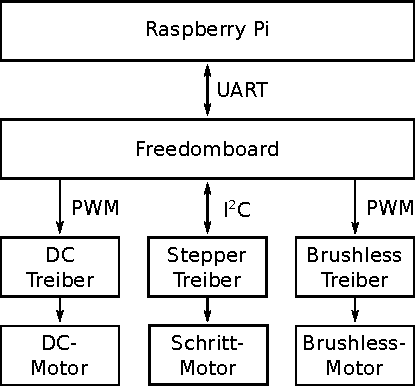
\includegraphics[scale=1]{../../fig/motor-control-overview.pdf}
	\caption{Schnittstellenübersich der Motoransteuerung}
\end{figure}

Die Software auf dem Freedomboard wird in der Programmiersprache C
implementiert. Als Entwicklungshilfe stehen zwei Entwicklungsumgebungen
des Herstellers Freescale Semicondutor zur Verfügung, einerseits CodeWarrior
und andererseits KinetisDesignStudio. Beide Entwicklungsumgebungen sind
an der Hochschule Luzern in Gebauch und verfügbar für die Benutzung.
